\documentclass[tikz,border=2pt]{standalone}
\usepackage{amsmath,amssymb}
\usepackage{tikz}

\begin{document}
% Illustrative instance: items 15, 30, 20, 35 with capacity 50. Total weight 100 gives the
% bound ceil(100/50) = 2, and the packing {15,35}, {30,20} attains it.
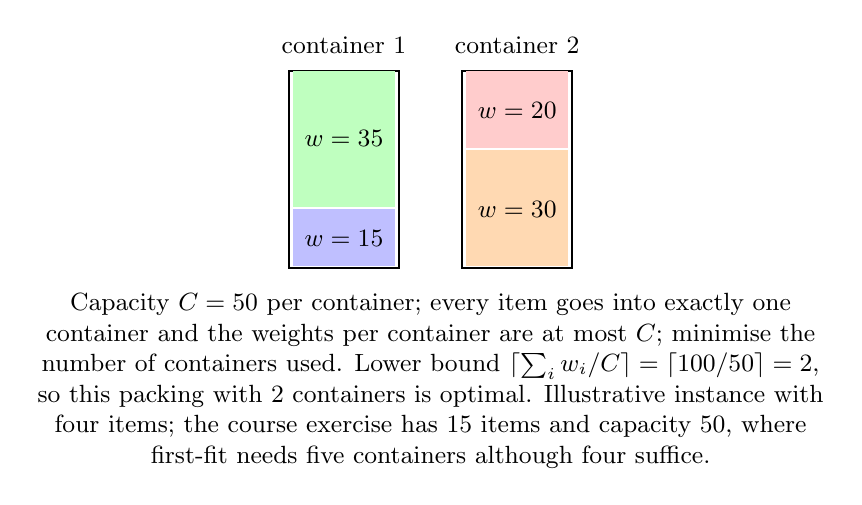
\begin{tikzpicture}[every node/.style={font=\small}, y=0.05cm]
	\foreach \x/\n in {0/1, 2.2/2} {
		\draw[thick] (\x,0) rectangle ({\x+1.4},50);
		\node[anchor=south] at ({\x+0.7},52) {container \n};
	}
	\fill[blue!25] (0.05,0.5) rectangle (1.35,15); \node at (0.7,7.5) {$w=15$};
	\fill[green!25] (0.05,15.5) rectangle (1.35,50); \node at (0.7,33) {$w=35$};
	\fill[orange!30] (2.25,0.5) rectangle (3.55,30); \node at (2.9,15) {$w=30$};
	\fill[red!20] (2.25,30.5) rectangle (3.55,50); \node at (2.9,40) {$w=20$};
	\node[anchor=north, align=flush center, text width=10cm] at (1.8,-4) {Capacity $C=50$ per container; every item goes into exactly one container and the weights per container are at most $C$; minimise the number of containers used. Lower bound $\lceil\sum_iw_i/C\rceil=\lceil100/50\rceil=2$, so this packing with $2$ containers is optimal. Illustrative instance with four items; the course exercise has $15$ items and capacity $50$, where first-fit needs five containers although four suffice.};
\end{tikzpicture}
\end{document}
